\section{Modelo de simulação}
\label{sec:model}

\subsection{Ferramenta utilizada}
A ferramenta escolhida para criar e executar o sistema dinâmico usado para simular o crescimento do número de utilizadores foi o \textit{Vensim}. De forma a aprender a usar esta ferramenta, foram seguidas as instruções apresentadas em \cite{vensim_youtube} e \cite{teacher_vensim}.

\subsection{Modelo criado}
O modelo criado em \textit{Vensim} está apresentado na figura \ref{model:vensim_model}. Este apresenta algumas similaridades com o segundo modelo apresentado no documento \cite{teacher_vensim} já que, sendo que a utilização duma aplicação depende da qualidade das \textit{features} que apresenta, alguns conceitos foram adaptados para este caso de estudo.

\begin{figure}[H]
   \begin{center}
       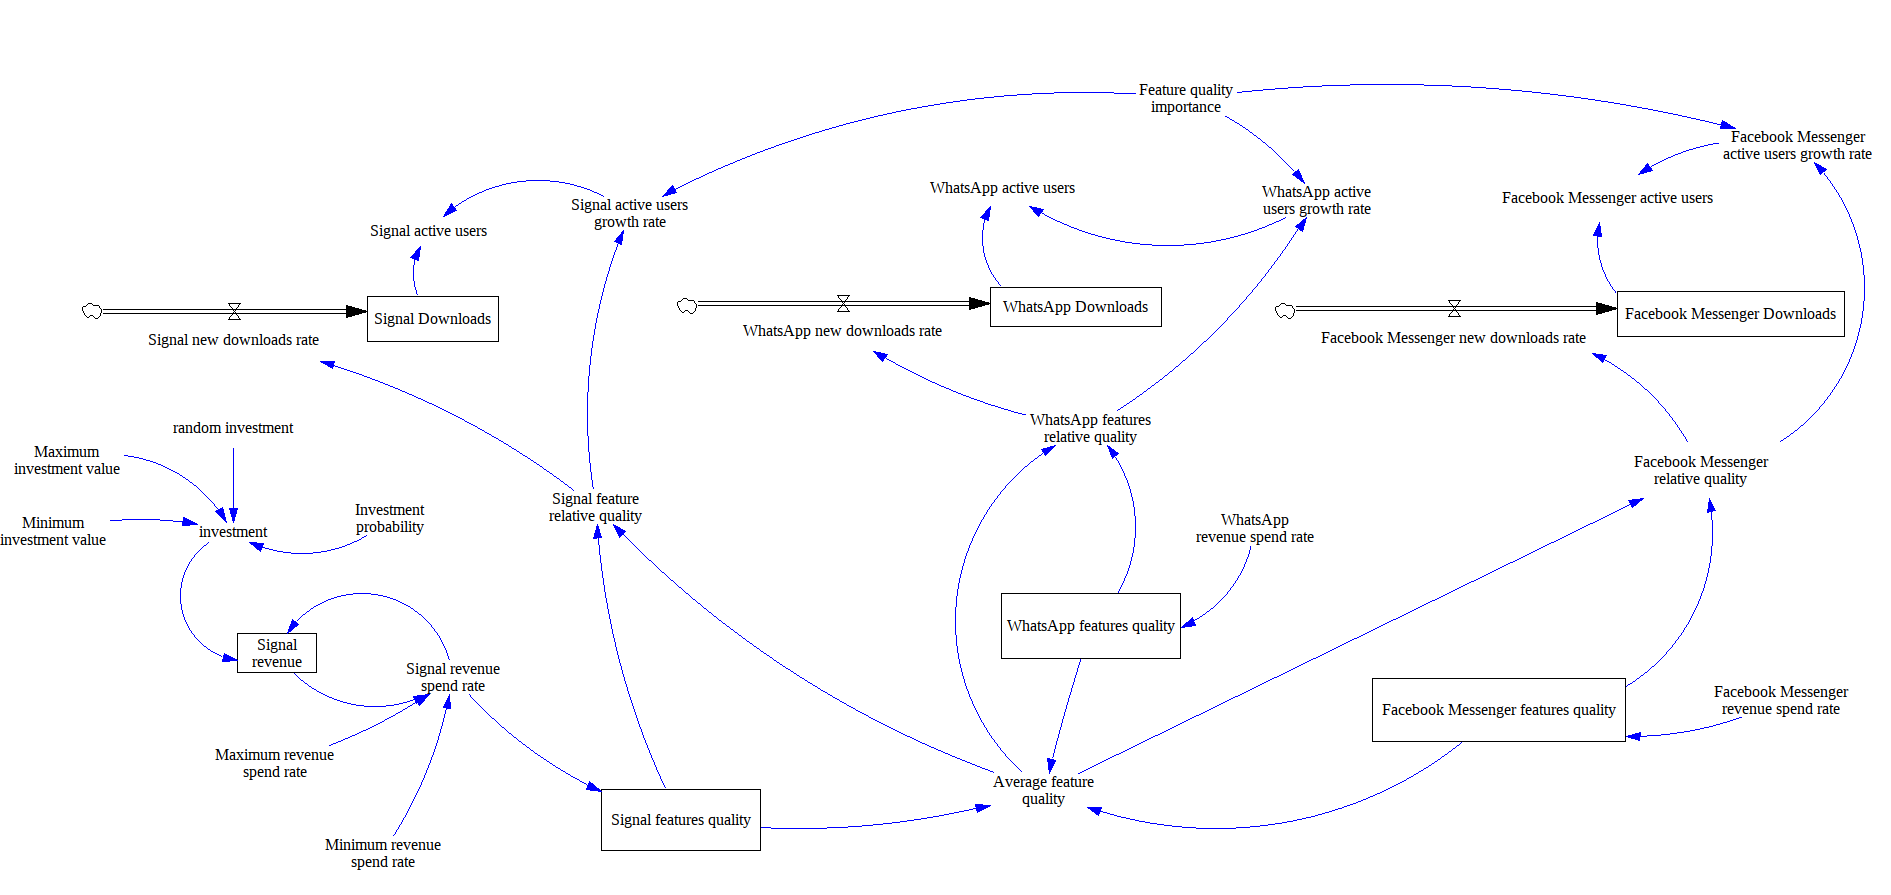
\includegraphics[width=17cm]{img/vensim_model.png}
       \caption{Modelo dinâmico criado em \textit{Vensim}.}
       \label{model:vensim_model}
   \end{center}
\end{figure}

Para a construção deste modelo, foram tidos alguns comportamentos verificados no passado do crescimento destes serviços em conta (ter em atenção que a unidade de tempo tida em conta neste modelo foi o \textit{Mês}):

\begin{itemize}
   \item Possíveis investimentos à \textit{Signal foundation}. Como explicado pelo fundador do \textit{Signal}, Moxie Marlinspike, o grande investimento de 50 milhões de dólares feito em 2018 pelo co-fundador do \textit{WhatsApp} foi um passo importante para aumentar o número de trabalhadores de 3 para atualmente 20. Com mais trabalhadores, foi possível criar novas \textit{features} já suportadas por outras aplicações concorrentes, como reagir a mensagens com \textit{emojis} (tal como no \textit{Facebook Messenger}) ou o envio de \textit{stickers}, sem nunca comprometer a segurança do serviço \cite{wired_signal}. Sendo assim, neste modelo foi tida em conta uma probabilidade de ocorrer um grande investimento como este. A seguinte equação demonstra como foi calculada a probabilidade usada no modelo:
   
   \begin{equation}
      \begin{split}
         P(\textit{investimento num dado mês}) & = \frac{1}{(\textit{número de anos até ocorrer o primeiro investimento})*12} \\
         & = \frac{1}{(2018-2014)*12} \\
         & = \frac{1}{48}
      \end{split}
  \end{equation}

  \item Relação entre número de \textit{downloads} e número de utilizadores ativos mensais. Para isso, foi feito o calculo apresentado pela equação \ref{calc:rel} tendo-se em conta os dados do \textit{WhatsApp} e do \textit{Facebook Messenger}, tendo-se obtido nos dois casos uma relação de 28\% de utilizadores ativos em relação ao número de \textit{downloads} feitos no \textit{Google Play}.
  
  \begin{equation}
      \label{calc:rel}
      \begin{split}
         Relacao = \frac{\textit{número de utilizadores ativos mensalmente}}{\textit{número total de downloads}}
      \end{split}
   \end{equation}

   Com isso em conta, foi executado o modelo criado múltiplas vezes com vários valores da variável \textit{Feature quality importance}, até aos valores iniciais das variáveis \textit{WhatsApp active users growth rate} e \textit{Facebook Messenger active users growth rate} apresentarem um valor apróximado a 0.28, de forma a possuir um modelo cujas condições inicias fossem parecidas às reais.

   \item Gastos mensais de cada um dos serviços. No caso do \textit{Signal}, os gastos mensais foram calculados tendo em conta os investimentos e a receita total que a \textit{Signal foundation} teve até ao momento. Nos outros dois serviços, foi tido em conta que são serviços geridos por grandes empresas, possuindo gastos bem definidos ao longo do tempo. Para além disso, no caso destas duas aplicações, foi tida em conta o investimento apresentado em \cite{whatsapp_craft} e foi feita uma estimativa dos gastos mensais desde o lançamento da aplicação até ao momento de acordo com esse investimento.
   
   \item Valores iniciais de \textit{download rate} e do número de \textit{downloads}. Quanto à \textit{download rate} foi tido em conta o número de \textit{downloads} diários que se verificavam à data de criação do modelo no \textit{Google Play}, multiplicados por 30 para ter o valor médio mensal. No caso do número de \textit{downloads} iniciais, foi usado o número de \textit{downloads} que cada uma das aplicações possuía à data da criação do modelo no \textit{Google Play}. Estes valores foram já apresentados neste documento na secção \ref{sec:market_presence}.
   
   \item Valor inicial do investimento tido no \textit{Signal}. O valor inicial de rendimento to \textit{Signal} é de 50 milhões de dólares dado investimento feito em 2018 pelo co-fundador do \textit{WhatsApp}.
\end{itemize}

A tabela \ref{tab:variables} ilustra os valores ou equações que cada variável possui no modelo final.

\begin{table}[h]

   \centering
   \begin{adjustbox}{width=1\textwidth}
   \begin{tabular}{|l|l|l|l|l|}
   \hline
   \textbf{Variável} & \textbf{Equação/valor} & \textbf{Unidades} & \makecell{\textbf{Valor} \\ \textbf{máximo}} & \makecell{\textbf{Valor} \\ \textbf{mínimo}} \\
   \hline
   INITIAL TIME & \textit{0} & \textit{Month} &  &  \\\hline
   FINAL TIME & \textit{120} & \textit{Month} &  &  \\\hline
   Average feature quality & \makecell[l]{\textit{(Facebook Messenger features quality + Signal features quality +} \\ \textit{WhatsApp features quality)/3}} & \textit{quality} &  &  \\\hline
   Facebook Messenger active users & \textit{Downloads*Facebook Messenger active users growth rate} & \textit{people}  &  &  \\\hline
   Facebook Messenger active users growth rate & \textit{Feature quality importance*Facebook Messenger relative quality} &  &  &  \\\hline
   Facebook Messenger Downloads & \textit{INTEG (Facebook Messenger new downloads rate, 4.52277e+09)} & \textit{people} &  &  \\\hline
   Facebook Messenger features quality & \textit{INTEG (Facebook Messenger revenue spend rate*20, 100)} & \textit{quality} &  &  \\\hline
   Facebook Messenger new downloads rate & \textit{4.56322e+07*Facebook Messenger relative quality} & \textit{people/Month} & 0 &  \\\hline
   Facebook Messenger relative quality & \textit{Facebook Messenger features quality/Average feature quality} &  &  &  \\\hline
   Facebook Messenger revenue spend rate & \textit{0.4} & \textit{million dollars/Month} & 0 & 1 \\\hline
   Feature quality importance & \textit{0.27} &  &  &  \\\hline
   investment & \makecell[l]{\textit{IF THEN ELSE(random investment < Investment probability, RANDOM 0 1()*} \\ \textit{(Maximum investment value - Minimum investment value) + } \\ \textit{Minimum investment value, 0)}} & \textit{million dollars} &  &  \\\hline
   Investment probability & \textit{1/48} &  & 0 & 1  \\\hline
   Maximum investment value & \textit{50} & \textit{million dollars} & 0 & 100 \\\hline
   Minimum investment value & \textit{10} & \textit{million dollars} & 0 & 50 \\\hline
   Maximum revenue spend rate & \textit{0.7} & \textit{million dollars} & 0 & 2 \\\hline
   random investment & \textit{RANDOM 0 1()} &  &  &  \\\hline
   Signal active users & \textit{Signal Downloads*Signal active users growth rate} & \textit{people} &  &  \\\hline
   Signal active users growth rate & \textit{Feature quality importance*Signal feature relative quality} & \textit{people/Month} &  &  \\\hline
   Signal Downloads & \textit{INTEG (Signal new downloads rate, 2.01246e+07)} & \textit{people} &  &  \\\hline
   Signal feature relative quality & \textit{Signal features quality/Average feature quality} &  &  &  \\\hline
   Signal features quality & \textit{INTEG (Signal revenue spend rate*20, 85)} & \textit{quality} &  &  \\\hline
   Signal new downloads rate & \textit{646740*Signal feature relative quality} & \textit{people/Month} & 0 &  \\\hline
   Signal revenue & \textit{INTEG (investment-Signal revenue spend rate, 50)} & \textit{million dollars} &  &  \\\hline
   Signal revenue spend rate & \makecell[l]{\textit{IF THEN ELSE(Signal revenue > 10, RANDOM 0 1()*(Maximum revenue spend rate -} \\ \textit{Minimum revenue spend rate) + Minimum revenue spend rate, 0.1)}} & \textit{million dollars/Month} &  &  \\\hline
   WhatsApp active users & \textit{WhatsApp Downloads*WhatsApp active users growth rate} & \textit{people} &  &  \\\hline
   WhatsApp active users growth rate & \textit{Feature quality importance*WhatsApp features relative quality} & \textit{people/Month} &  &  \\\hline
   WhatsApp Downloads & \textit{INTEG (WhatsApp new downloads rate, 5.33992e+09)} & \textit{people} &  &  \\\hline
   WhatsApp features quality & \textit{INTEG (WhatsApp revenue spend rate*20, 100)} & \textit{quality} &  &  \\\hline
   WhatsApp features relative quality & \textit{WhatsApp features quality/Average feature quality} &  &  &  \\\hline
   WhatsApp new downloads rate & \textit{7.5802e+07*WhatsApp features relative quality} & \textit{people/Month} & 0 &  \\\hline
   WhatsApp revenue spend rate & \textit{0.4} & \textit{million dollars/Month} & 0 & 1 \\
   \hline
   \end{tabular}
   \label{tab:variables}
   \end{adjustbox}
   \caption{Equações e variáveis utilizadas}
\end{table}
